% This is a template for BU-ECE Technical Report.
%
% Depending on report content and author preference, a BU-ECE report may be
% in one of the two following styles:
%
%   - genuine report based on ``report'' style, i.e., with chapters, much like
%     a thesis; can be single- or double-sided,
%
%   - report based on ``article'' style, i.e., with no chapters (only sections,
%     subsections, etc.), much like a journal or conference paper; can be
%     single- or double-sided.

% =====================================================================

%\documentclass[12pt]{report}          %Single-sided report style (chapters)
%\documentclass[12pt,twoside]{report}  %Double-sided report style (chapters)
%\documentclass[12pt]{article}         %Single-sided article style (no chapters)
\documentclass[12pt,oneside]{article} %Double-sided article style (no chapters)

\usepackage{bu_ece_report}

% In case an adjustment of vertical or horizontal margins is needed
% due to particular LaTeX/dvips or OS installation, you can uncomment
% and edit the following definitions.
% -------------------------------------------------------------------
%\topmargin       0.00 in
%\oddsidemargin   0.50 in
%\evensidemargin  0.00 in

\begin{document}

% Definitions.
% ------------
\buecedefinitions%
        {Room Occupancy sensing using a thermal tripwire}
        {Occusense: Final Report}
        {Janis Intoy and Emily Lam}
        {May 5, 2017}
        {2017-01} % Number of the report (four year digits and number) What is the number supposed to be???????? NO IDEA!!

% Box with title to fit the opening in the cover
% (adds an empty page in double-sided printing mode).
% ---------------------------------------------------
\buecereporttitleboxpage

% Title page
% (adds an empty page in double-sided printing mode).
% ---------------------------------------------------
\buecereporttitlepage

% Special page, e.g., if the report is restricted or
% to whom it is dedicated, etc., otherwise skip.
% (adds an empty page in double-sided printing mode).
% ---------------------------------------------------
%\bueceprefacepage{Here comes a special preface page. For example, if the report
%is restricted, then a suitable note can be included. This page can also be used
%to indicate to whom the document is dedicated, etc.}

% Report summary; max. 1 page.
% (adds an empty page in double-sided printing mode).
% ---------------------------------------------------
\pagenumbering{roman}
\setcounter{page}{1}
\buecereportsummary{
A large part of a building's efficiency depends on the efficiency of its HVAC (Heating Ventilation \& Air Conditioning) system, which can be improved with automatic adjustments based on room occupancy level. As thus, accurate prediction of the number of people in a room is needed. In order to estimate a room's occupancy level, the Occusense Senior Design team has created a privacy-preserving, low resolution, thermal sensor system to capture temperature images of people walking through the doorways. This project uses that information coupled with a background prediction algorithm and optical flow analysis to predict the direction of motion of the people passing through and keep a continuous count of the number of people in the room. \\ \\ We test our algorithm on people moving in and out, people lingering at the door, people rushing through the door, and multiple people passing together through the door. Our algorithm was not successful for people passing together through the door. Final results are 90\% in classification and an error of $\pm$3 in the occupancy count after 10 people pass through the door in either direction.}

% Table of contents, list of figures and list of tables.
% ``\bueceemptypage'' adds empty page in double-sided
% printing mode and performs ``\clearpage'' in single-sided
% mode.
% ------------------------------------------------------
\tableofcontents\bueceemptypage
\listoffigures\bueceemptypage
\listoftables\bueceemptypage

% Switch on running headers for the report:
%   odd pages  - title (lowercase); if too long, use
%                the first few words followed by ``...'',
%   even pages - last names of the authors.
% -------------------------------------------------------
\buecereportheaders

% Introduction.
% -------------
\pagenumbering{arabic}
\setcounter{page}{1}

\section{Introduction}  % Article style
%\chapter{Introduction}  % Report style
In modern efficient buildings, controlling the HVAC system preemptively can be a huge cost saver. Therefore, Occusense, a senior design team at Boston University, is working towards developing sensing technology and algorithms to continuously keep count of the number of people in a room. This way, the system can adjust system parameters, such as ventilation, accordingly, before feedback sensing technology can detect abnormalities in the air quality of a room. There are a number of ways to detect occupancy, such as using a fisheye camera to count the number of people in a frame. However, this project assumes a tripwire methodology, that is if a room has a low number of entry points, counting people can be done at the entries based on if someone or something is entering or leaving the room. As such, continuous knowledge of the number of people in a room is achieved as a running tally. The Occusense team has implemented a low resolution thermal sensor with a field of view of 30$^\circ$x120$^\circ$ positioned at the top of the door frame and looking perpendicularly down, Figure~\ref{door}. It is capable of capturing a 4x16 pixel array of temperatures at frame rates of 8-12Hz. Using this information, our project develops an algorithm to count the number of people entering or leaving a room. Specifically, this algorithm will 1) detect the presence of a moving person in the frame, 2) determine the direction of motion of the person, and 3) keep count of the total number of people in a room.

\begin{figure}[!htb]
\centering
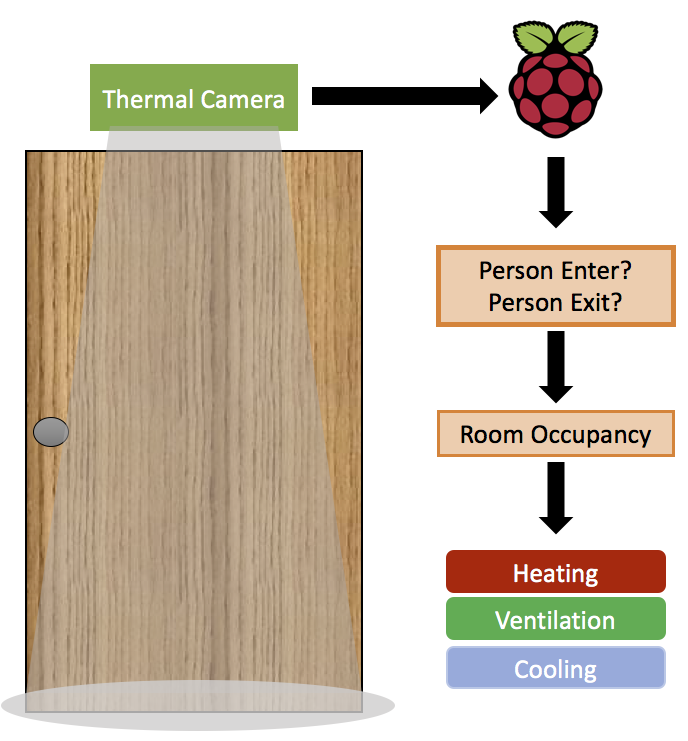
\includegraphics[scale=0.4]{images/door.png}
\caption{Overarching system diagram. Our work focuses on the orange boxes.}
\label{door}
\end{figure}

% Following sections, subsections, etc.
% -------------------------------------
\section{Literature Review}  % Article style
%\chapter{Starting chapter}  % Report style
% Briefly review the literature discussing some other approaches proposed to solve the problem (if any).
Many background subtraction algorithms have been developed to detect changing pixels in a series of images.
A brief review of simple background subtraction methods can be found in \cite{Piccardi04} and
more common change detection algorithms in \cite{Goyette14}.
The most successful amongst these incorporate a background model into the algorithm. The use of a model
allows for thresholding of probabilities instead of pixel intensities and is therefore more robust to some variation
in the background scene. In addition, foreground models can improve the sensitivity of the change detectors 
\cite{Elgammal02}. McHugh et al. suggested a foreground model algorithm that is more general as it
is based on spatial neighborhoods. To further improve the discrimination, they also suggest a Markov model
so that labels are more spatially coherent
\cite{Mchugh09}.
\\ \\
We also looked into algorithms for determining optical flow. Optical flow describes the direction elements in an image move or change with space and time from frame to frame, usually in a vector form. There are three overarching approaches for determining optical flow: a feature-based approach, a correlation-based approach, and a gradient-based approach. For our project we consider the gradient-based approach on foreground elements so that only the foreground elements are put through the gradient-based optical flow algorithm when determining object motion. While this method relies on background subtraction for foreground selection, it does not require prior training. The gradient-based optical flow algorithm models gradients based on partial derivatives for each pixel intensity with respect to space and time, as each pixel's intensity will have a change in both the x-direction, y-direction, and time \cite{Smith97}.

\section{Problem Statement and Proposed Solution}  % Article style
%\section{Early section}  % Report style
% Describe the problem in detail, and the solution proposed, including assumptions, constraints, math formulas, algorithms,
% etc.
Our project aims to keep track of the number of people in a room based on the tripwire methodology. Our approach breaks the problem into three parts: 1) detect a person in the doorway, 2) determine the direction of motion of the person, 3) classify the motion and track the total number of people in a room.

\subsection{Person Detection}
In order to accomplish this
we make several assumptions about the acquired data. First, we assume that the background has slow temporal dynamics.
Second, we assume that the data starts with some number of background-only frames. For business and residential 
buildings this is likely true if they close for the night. Finally, we assume that the noise in the 
surface temperature measurements is independent of the signal.
Here we propose two background subtraction methods to detect a person or persons in the frame. 
One method to detect foreground in each frame is to model the background temperatures of each pixel as a 
Gaussian which is updated with each new frame. The parameters of the background model are updated when 
the current pixel is labeled as background:
$$\mu_t [\mathbf{n}] = \rho I_t [\mathbf{n}] + (1-\rho)\mu_{t-1} [\mathbf{n}]$$
$$\sigma_t^2 [\mathbf{n}] = (I_t [\mathbf{n}] - \mu_t [\mathbf{n}])^2 \rho + (1-\rho)\sigma_{t-1}^2 [\mathbf{n}]$$
where $I_t [\mathbf{n}]$ is the pixel temperature at position $ [\mathbf{n}]$ 
and $\mu_t$ and $\sigma_t^2$ are the mean and variance
of the gaussian in frame $t$. A Markov model can be applied to improve the spatial coherency of foreground labels:
a pixel surrounded by foreground pixels has a low threshold since it is likely also foreground. Therefore,
a pixel is labelled as foreground when
$$\frac{I_t [\mathbf{n}] - \mu_{t-1} [\mathbf{n}]}{\sigma_{t-1} [\mathbf{n}]} >_\mathcal{F} \theta \exp((Q_\mathcal{B} [\mathbf{n}] - Q_\mathcal{F} [\mathbf{n}]) / \gamma)$$
where $\theta$ is an initial threshold (\# of standard deviations), $Q_\mathcal{B}[\mathbf{n}]$ and $Q_\mathcal{F}[\mathbf{n}]$ are the number
of background and foreground pixels neighboring the pixel at position $ \mathbf{n}$ respectively, and $\gamma$ is a parameter that changes 
the influence of the Markov model on the threshold.
\\ \\
The second proposed solution is inspired primarily by the foreground-adaptive background subtraction described in
\cite{Mchugh09}.
The background can be modeled by a probability density function estimated at each pixel location $\mathbf{n}$
from the $N$ most recent pixels that were labeled as background:
$$P_\mathcal{B}\left(I_t [\mathbf{n}]\right) = \frac{1}{N}\sum_{i \in \mathcal{B}_t[\mathbf{n}]} \mathcal{K}
	\left(I_t[\mathbf{n}] - I_i[\mathbf{n}] \right)$$
where 
$B_t[\mathbf{n}]$ are the $N$ previous time indices at which the pixel located at $\mathbf{n}$ was labeled
background, and $\mathcal{K}$ is a zero-mean Gaussian with variance $\sigma^2$. Thresholding these probabilities
with threshold $\theta$ gives an initial classification of pixels into background or foreground.
\\ \\
The development of the foreground model follows a similar formulation, but the summation is over
pixels in the neighborhood of $\mathbf{n}$ that already have been labeled as foreground. The
ratio of the probability density functions $P_\mathcal{B}$ and 
$P_\mathcal{F}$ can be thresholded to determine new labels for each pixel. Furthermore,
the number of foreground neighbors a pixel has can be used to adjust the threshold. The more foreground
neighbors a pixel has the easier it is to be labeled as foreground. This will contribute to the spatial
coherence of the labels. Thus, a pixel is labeled as background if
$$\frac{P_\mathcal{B}(I_t[\mathbf{n}])}{P_\mathcal{F}(I_t[\mathbf{n}])} > \theta \exp \left(\frac{1}{\gamma} 
	(Q_\mathcal{F}[\mathbf{n}] - Q_\mathcal{B}[\mathbf{n}] )\right)$$
where $\gamma$ is a parameter to control how strongly the threshold
adapts. The thresholding step can be done iteratively as labels are updated in each step.

\subsection{Direction Discrimination}
After determining the foreground from the background, we look at determining the direction of flow of the foreground elements. We do this by taking the foreground elements only, setting the background elements to zero, and applying a gradient-based optical flow algorithm. This can be modeled as described in \cite{Smith97}:
$$\frac{\partial I}{\partial x}\frac{\partial x}{\partial t}+\frac{\partial I}{\partial y}\frac{\partial y}{\partial t} + \frac{\partial I}{\partial t}=0$$
Since we are only concerned with the vertical velocity, i.e. a person walks through the door frame and the lateral motion is trivial, the previous equation can be written as
$$v_y = - \frac{\frac{\partial I}{\partial t}}{\frac{\partial I}{\partial y}}$$
where a large $v_y $ would correspond to a lot of motion in that direction. 
\begin{figure}[!htb]
\centering
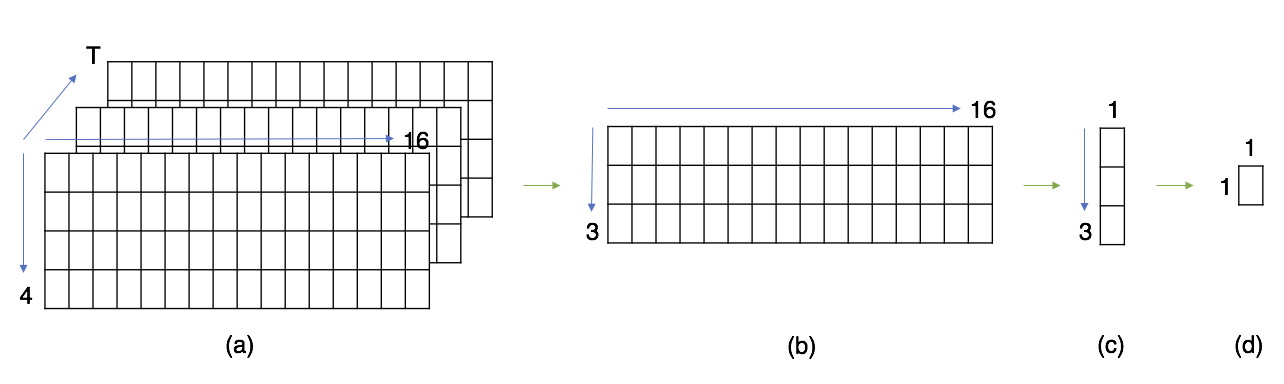
\includegraphics[scale=0.3]{images/matrix.png}
\caption{(a) raw 4x16xT matrix, $I(i,j,t)$ (b) 3x16 spatial gradients matrix at time $t$, $A(i,j,t)$, (c) 3x1 row averaged spatial gradients at time $t$, $B(i,t)$, (d) row and column averaged spatial gradients at time $t$, $C(t)$.}
\label{matrix}
\end{figure}
In our system of 4x16 pixels array, we only consider the foreground pixels with the background elements set to zero. We generate a spatial gradient matrix consisting of 3x16 pixels to take the boundary condition into account to get matrix, $A(j,i,t)$, at time $t$, as follows: $$A(i,j,t) = I(i+1,j,t) - I(i,j,t) : i = 1, . . ., 3, j = 1, . . ., 16$$ Next, we perform two averages, we average the rows to find the overall spatial gradient of the row, $B(i,t)$, at time $t$, as follows: $$B(i,t) = \frac{1}{16}\sum_{j=1}^{16}A(i,j,t) : i = 1, . . .,3$$ Then we average those row averages together to obtain an overall spatial gradient for the entire matrix at time $t$, as follows: $$C(t) = \frac{1}{3}\sum_{i=1}^{3}B(i,t)$$ The temporal gradients are taken from $C(t)$ between consecutive frames, which also has spatial information embedded in it. As an example, the final velocity for two consecutive frames is then calculated as: $$v_y(t) = \frac{C(t)}{C(t+1)-C(t)}$$ which is used to determine the optical flow of the foreground which in turn determines whether a person is walking into or out of the room. 

\subsection{Classifier and Counter}
The classier determines when an event starts and stops based on the background subtraction algorithm. The counter then compares the overall spatial gradients, $C(t)$, at different times, not necessarily consecutive frames, during each event and increments the overall counter accordingly. In addition, it takes into account edge cases for determining between noise and data for single-frame events.

\newpage

\section{Implementation}  % Article style
%\chapter{Another chapter}  % Report style
% Describe how you have implemented the proposed solution; include the source code in the appendix.
The current implementation of the algorithm is in Matlab. The data, code, and documentation is available
on github: https://github.com/janisirene/Occusense.
 The three parts of the algorithm, Figure~\ref{threestep},
are implemented
separately and can be run in sequence to output a single room occupancy number. We define an event as a series of consecutive frames with detected motion as determined by the background subtraction algorithm.
\begin{figure}[htb] % implentation flow
\centering
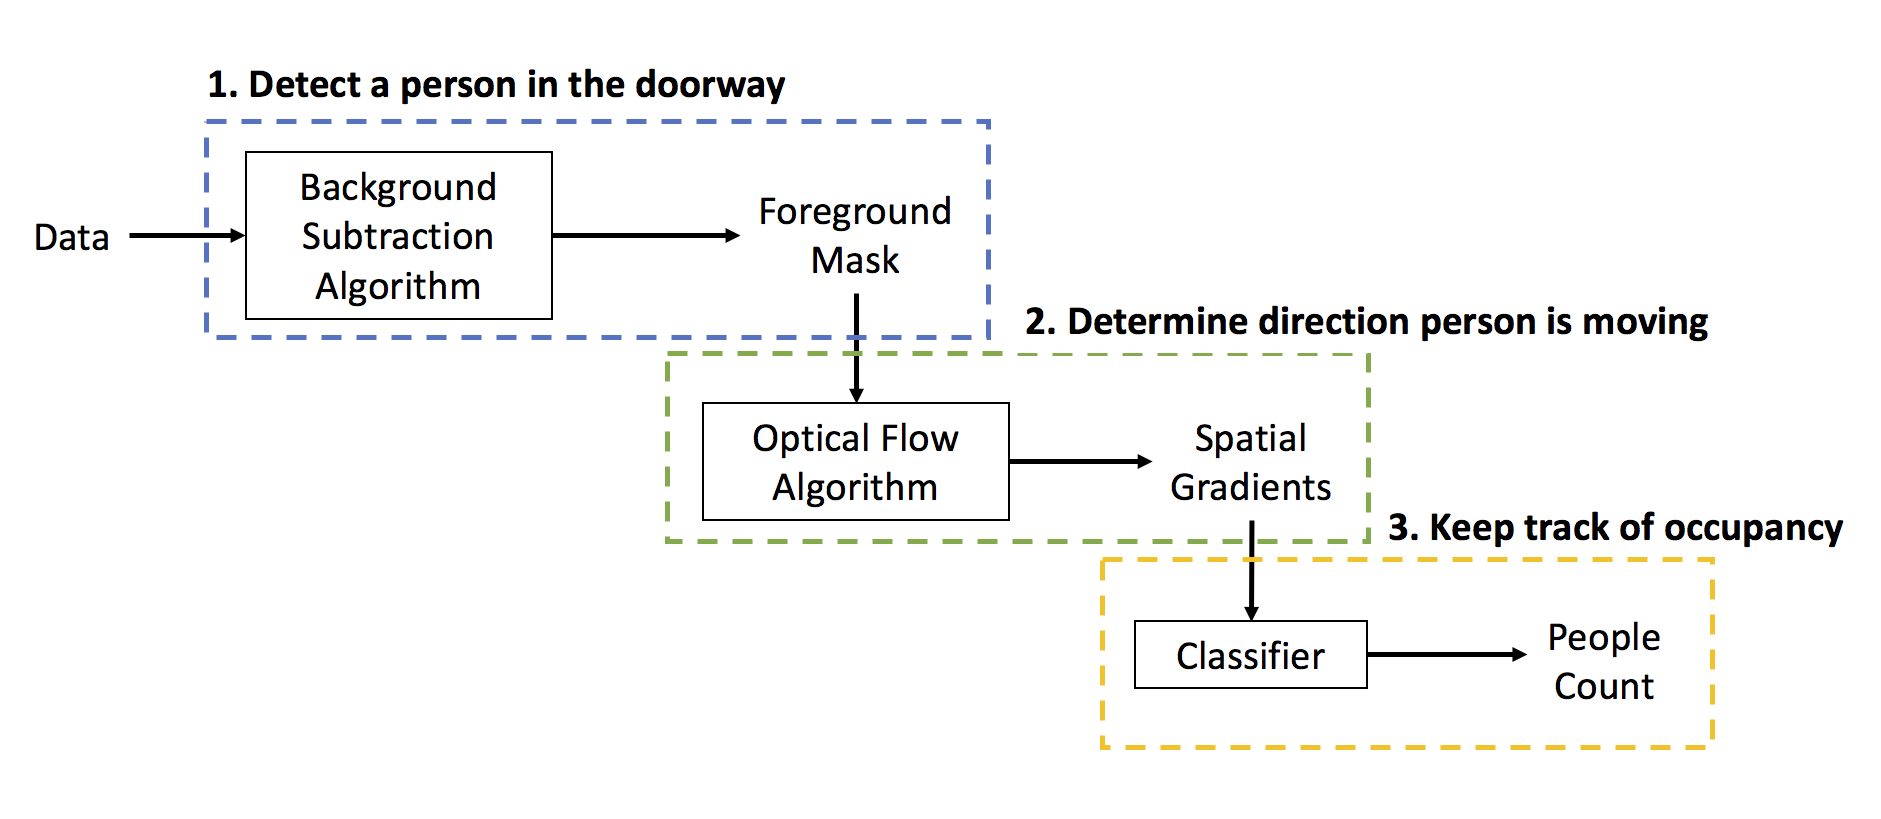
\includegraphics[scale=0.2]{images/threestep.png}
\caption{Three-step implementation.}
\label{threestep}
\end{figure}

\subsection{Data Acquisition}  % Article style
%\section{New section}  % Report style
The Occusense team provided labelled data which consisted of several second recordings of 
one or two people passing through the doorway. We separated this data into 86 periods of
background (no body present in frame) and 55 periods with foreground motion (body present in frame).
In addition to the labelled data from the senior design team, we acquired several trials of realistic but more
difficult situations. This includes a person lingering in the doorway, a person rushing out the door and back in, and multiple people passing through
the door in quick succession.
\\ \\
The data was recorded into text files at a rate of 8-12Hz. The labeled data was recorded at 8Hz
by the Occusense team and the difficult situations data was recorded at 12Hz.

\subsection{Person Detection}
Janis implemented both proposed background subtraction algorithms in backgroundSubtractionSimple.m 
(running gaussian) and backgroundSubtraction.m (kernel-based approach).
They take as input a structure of parameters
and a 3-D array of temperatures over the two spatial and one temporal dimensions. 
The best parameter ranges are described in Table \ref{bs_paramstable}.
This implementation could
be modified to run in real time and, depending on the size of the history for the computation of the background
PDF, would not require too much memory. The output of this function is a binary array of pixel labels 
(red dots in Figure~\ref{foregroundexample}). Motion events are identified by
thresholding the total number of detected pixels (Figure~ \ref{abs_example}).
\begin{table}[htb]\begin{tabular}{|clr|clr|}
\hline
\multicolumn{3}{|c|}{Foreground Adaptive} & \multicolumn{3}{|c|}{Running Gaussian Average}\\
\hline
& Description & Good Range & & Description & Good Range\\
\hline
$N$ & \# background frames & 10-30 & $N$ & \# background frames & 10-30\\
$\sigma$ & std of gaussian kernel & 0.4-0.6 & $\rho$ & size of temporal window & 0.01\\
$\gamma$ & influence of MRF & 0.2 - 0.8 & $\gamma$ & influence of MRF & $>1$\\
$N_\eta$ & neighborhood order & 1 & $N_\eta$ & neighborhood order & 1\\
$it$ & labelling iterations & 3 & $it$ & labelling iterations & 3\\
 &  &  & $\theta$ & threshold & 2.5\\
\hline
\end{tabular}
\caption{Good parameter ranges for background subtraction algorithms.}
\label{bs_paramstable}
\end{table}

\begin{figure}[htb] 
\centering
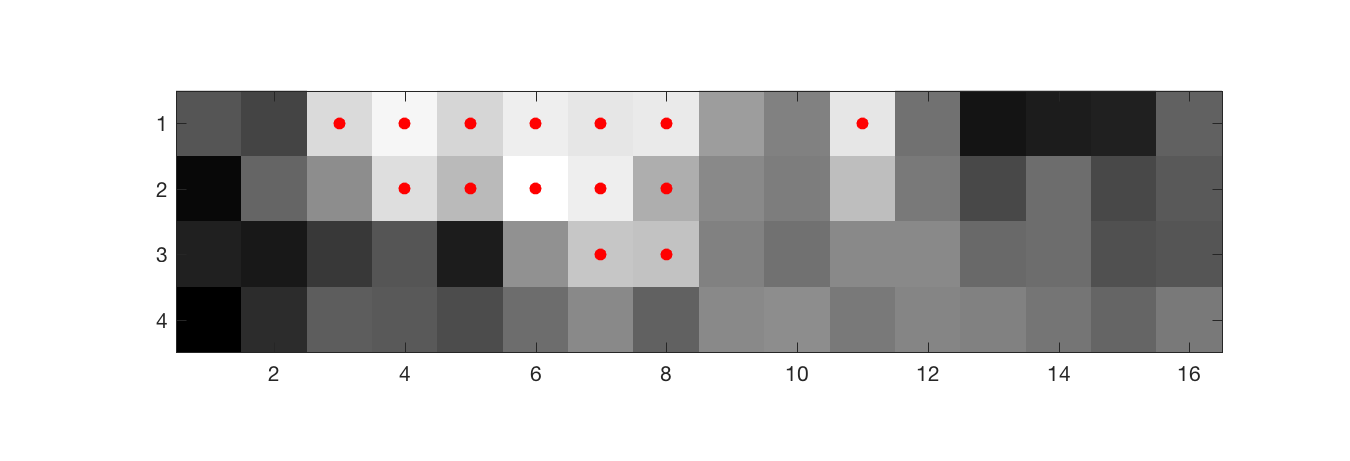
\includegraphics[scale=0.45]{images/foreground_example.png}
\caption{Example of detected foreground pixels.}
\label{foregroundexample}
\end{figure}

\begin{figure}[!htb]  % # detected foreground pixels / frame
\centering
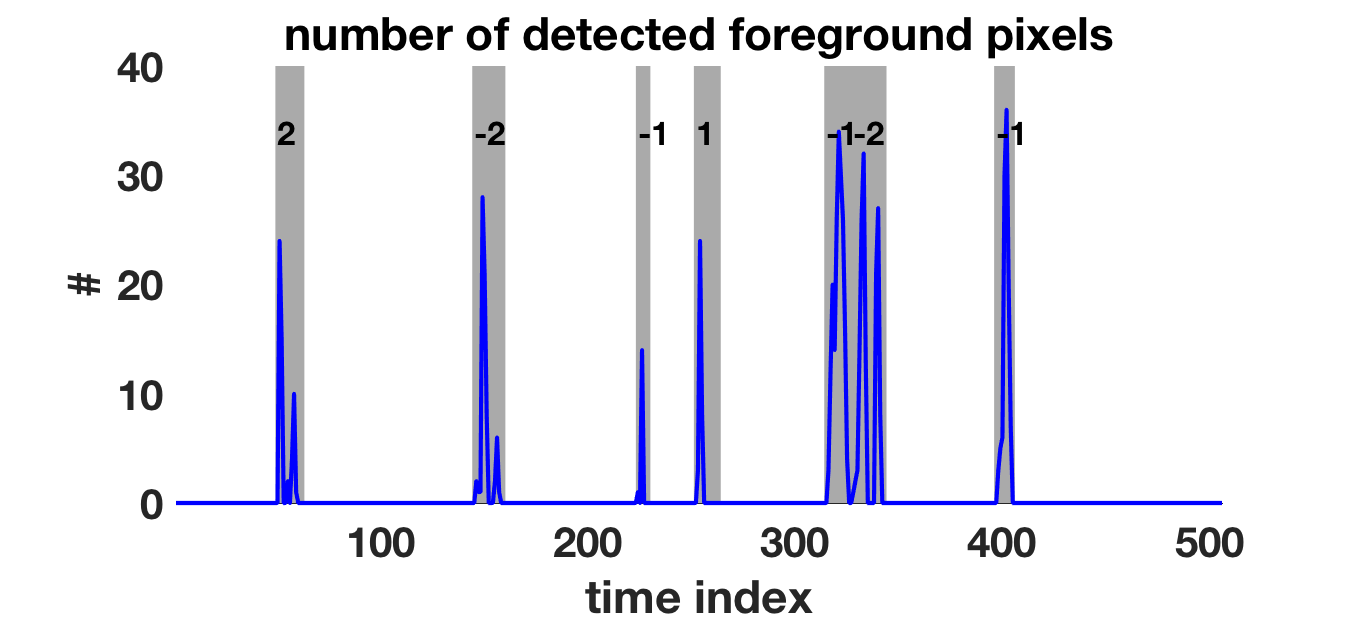
\includegraphics[scale=0.45]{images/abs_example.png}
\caption{Example of total number of foreground pixels in each frame compared to 
ground truth events in gray.}
\label{abs_example}
\end{figure}


\subsection{Direction Discrimination}
Emily implemented this algorithm in the file opticalflow.m. It takes as input a 3-D array of temperatures over the two spatial and one time dimensions. This can be the raw information provided by the sensors or a masked foreground-only version that has already undergone background subtraction. This function returns spatial gradients in various forms: for individual pixels, $A(i,j,t)$, (Figure~\ref{opflw}), averaged across rows, $B(i,t)$, and averaged per frame $C(t)$. This information is passed to pCounter.m to perform final temporal gradients, direction decisions, and track occupancy. This implementation could be modified to run in real time to follow the background subtraction function.
\begin{figure}[htb]
\centering
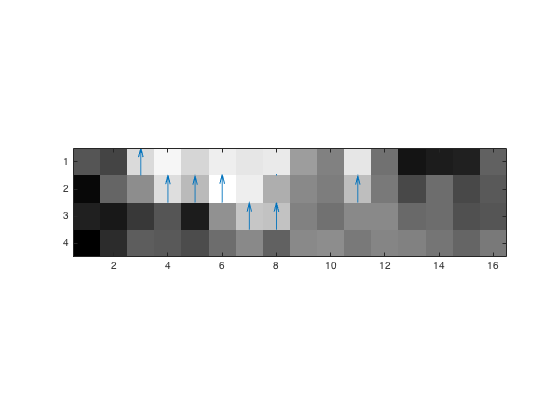
\includegraphics[scale=0.52]{images/quiver_gradients.png}
\caption{Example of optical flow vectors.}
\label{opflw}
\end{figure}


\subsection{People Count}
Janis and Emily implemented this algorithm in the file pCounter.m. This files takes the output of the opticalflow.m, a series of vertical gradients over time, and averages them per a frame and calculates the temporal gradients based on the first and and last time frame as the optical flow information for the frames corresponding to the middle of an event are too noisy. The direction is then decided based on this information. This function also decides when single-frame events are considered noise are not based on the mean number of foreground pixels. If there are less than 4 foreground pixels, the frame is considered to be noise and discarded. In addition, this information is used to determine when an event starts and stops.

\section{Experimental Results}  % Article style
%\chapter{Final chapter}  % Report style
% Describe the experiments you have conducted and the results you have obtained. Are you results consistent
% with your original goals?
Algorithms were tested on labelled data that consisted of random concatenations of the 
periods of background and foreground so that they resembled data collected
over an extended period of time. The temperatures of the individual periods were biased
to ensure continuity between frames. Also, since all of the data came from the same
setup where the sensor was on the inside of the room, individual periods were randomly flipped
vertically to remove the directional bias.

\subsection{Background Subtraction}  % Article style
The background subtraction results are shown as ROC curves (Figure~\ref{roc}).
The kernel-based method
had overall better performance than the parametric method achieving hit rates of over 90\% for the best
parameter sets with negligible false alarms in detecting a person in the frames. Most misses occurred
because of spontaneous rapid changes in temperature of background pixels. These occur infrequently
in the actual data, but also arise when true foreground pixels are mislabelled and bias the background model, for 
example at the edges of the foreground person. The effects of this are seen in Figure~ \ref{abs_example}, where
the second peak in an event is sometimes much lower than the preceding one.

\begin{figure}[htb]
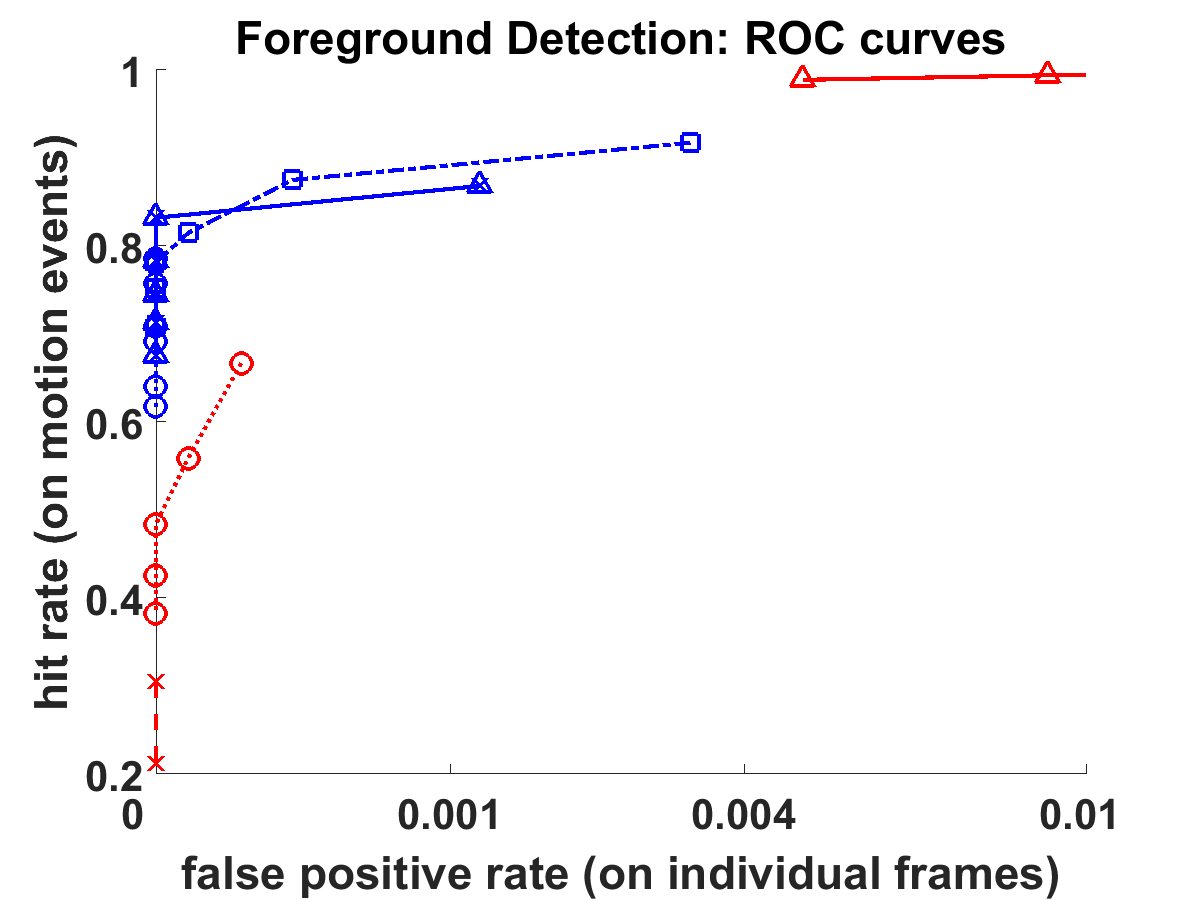
\includegraphics[scale=0.4]{images/roc.png}
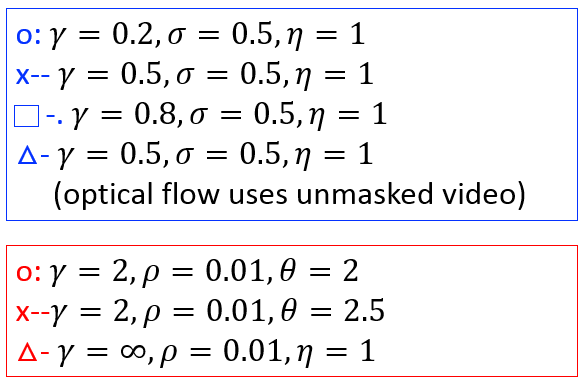
\includegraphics[scale=0.4]{images/legend.png}
\caption{ROC curves of detecting motion events using different parameters for the two proposed
background subtraction algorithms.}
\label{roc}
\end{figure}

\subsection{Direction Discrimination}  % Article style
The direction discrimination works for all cases we tried except for multiple people walking in together. For the simple case of two people walking out, Figure~\ref{twoout}, the background subtraction algorithm correctly identifies two events, and the direction is easy to discriminate from the optical flow. For lingering at the door, Figure~\ref{linger}, because the noisy information in the middle frames is ignored, this also works well with our algorithm. In the case of someone running out and in quickly, Figure~\ref{run}, again our algorithm is successful in determining the direction and successfully determines single frame events as motion versus noise. However, in the case where the background subtraction algorithm fails to detect individual people as individual events, the direction discrimination fails because it does not consider the middle frames in its decision, Figure~\ref{together}. This could be remedied by taking into account the middle frames and employing peak counting or zero-crossing analysis. However, since the middle frames provide noisy information as seen in the lingering example, this information cannot be relied on when counting the number of people entering or leaving. Overall, the direction discrimination works well, Figure~\ref{dirclass}, and the major result in error is due to the error in the background subtraction algorithm.

\begin{figure}[htb]
\centering
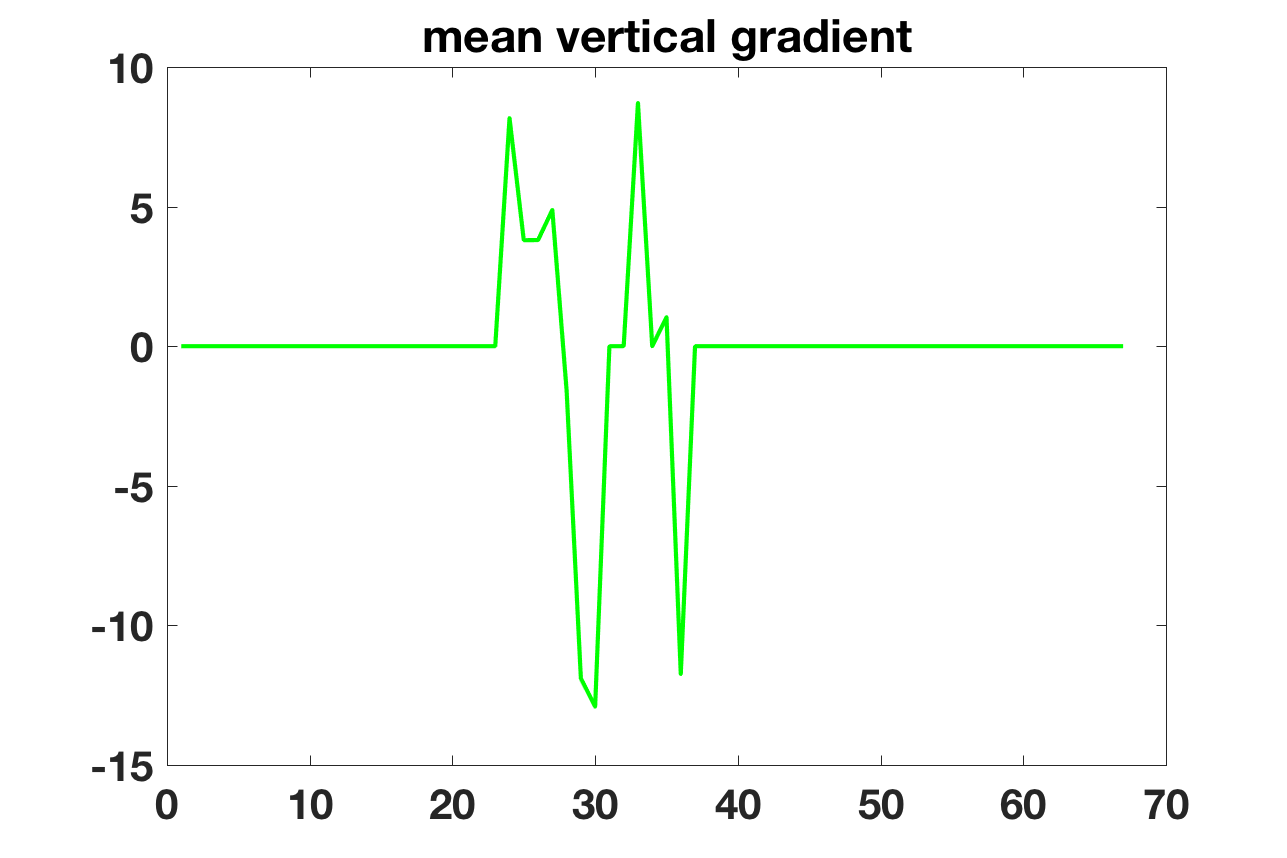
\includegraphics[scale=0.52]{images/two_out.png}
\caption{Mean vertical gradient for two people walking out.}
\label{twoout}
\end{figure}

\begin{figure}[!htb]
\centering
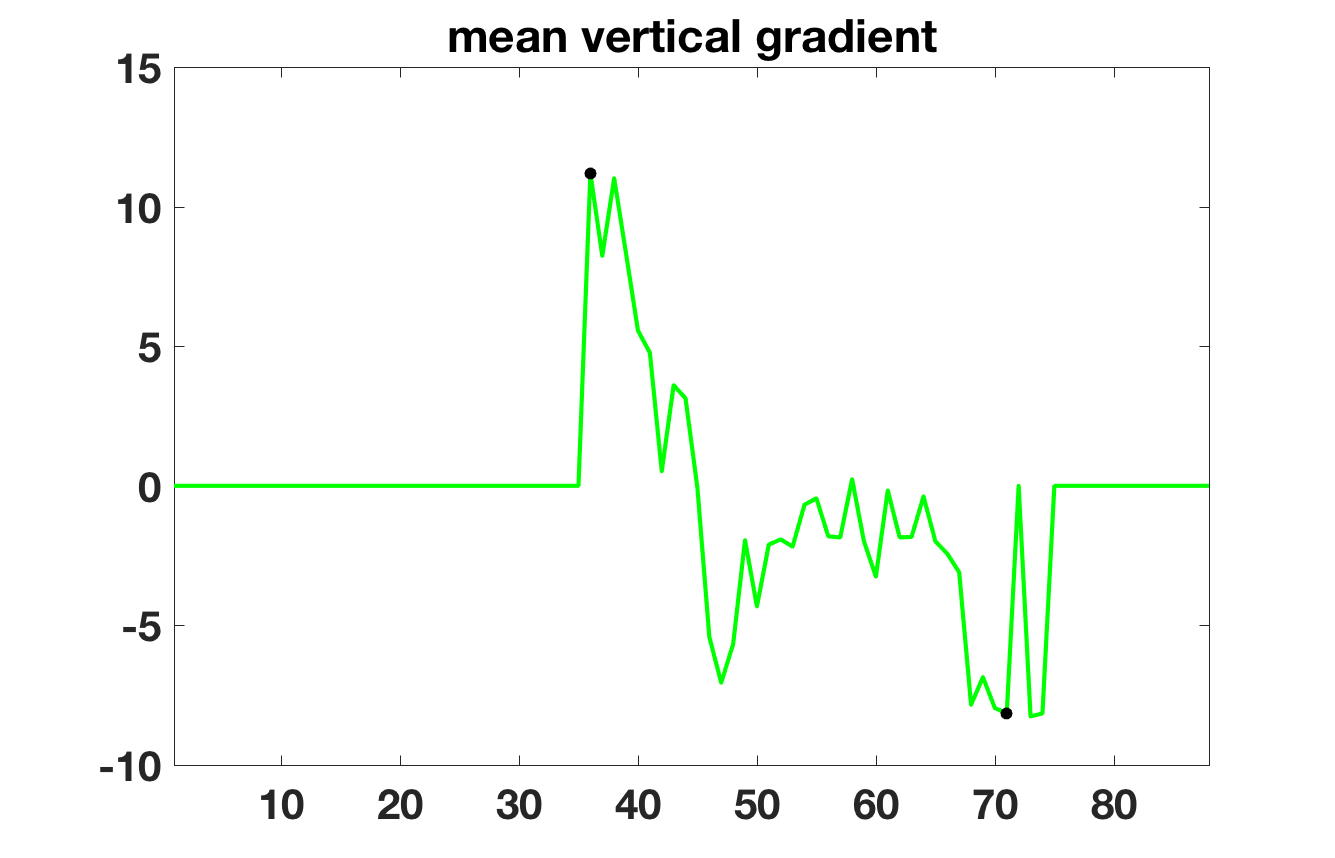
\includegraphics[scale=0.52]{images/lingerThrough.png}
\caption{Mean vertical gradient for lingering through the door.}
\label{linger}
\end{figure}

\begin{figure}[!htb]
\centering
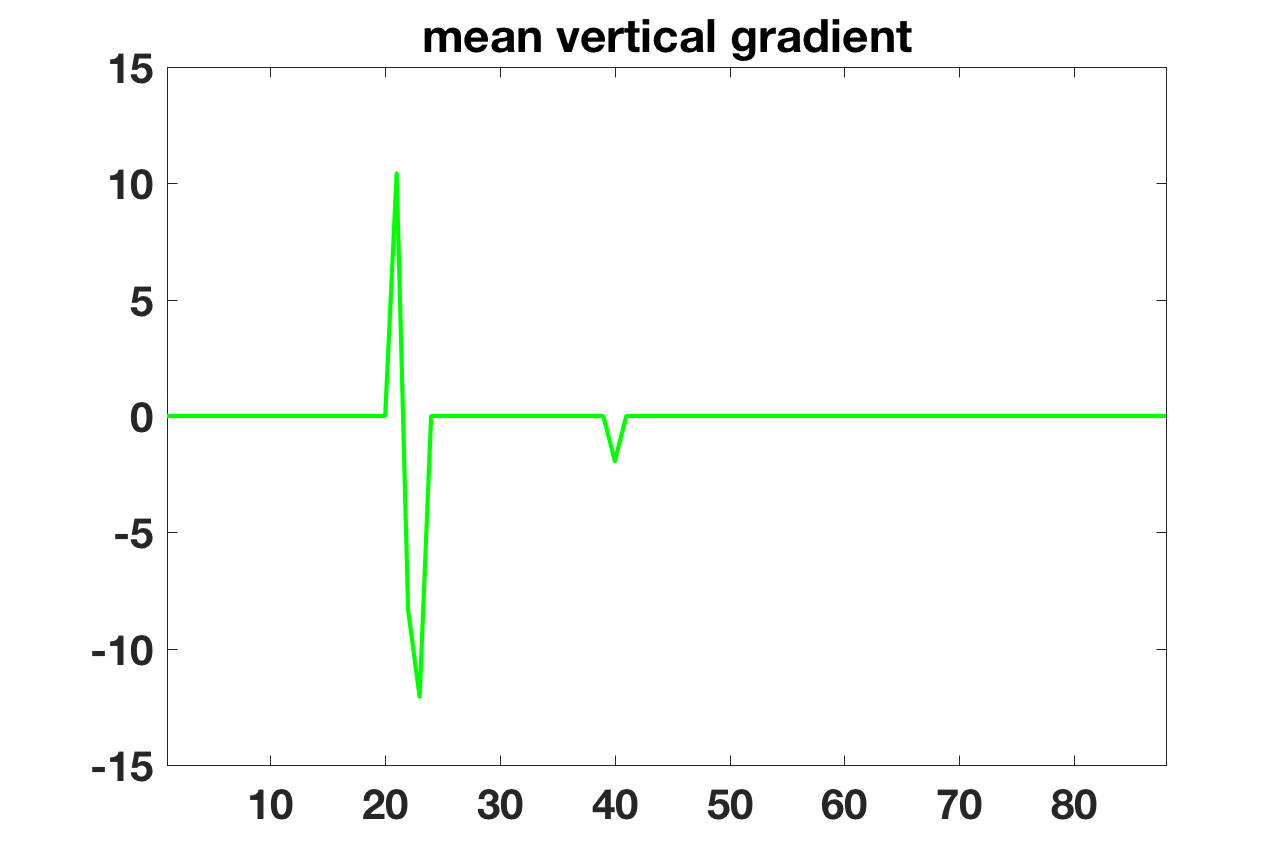
\includegraphics[scale=0.52]{images/runoutandin.png}
\caption{Mean vertical gradient for running out and in through the door.}
\label{run}
\end{figure}

\begin{figure}[!htb]
\centering
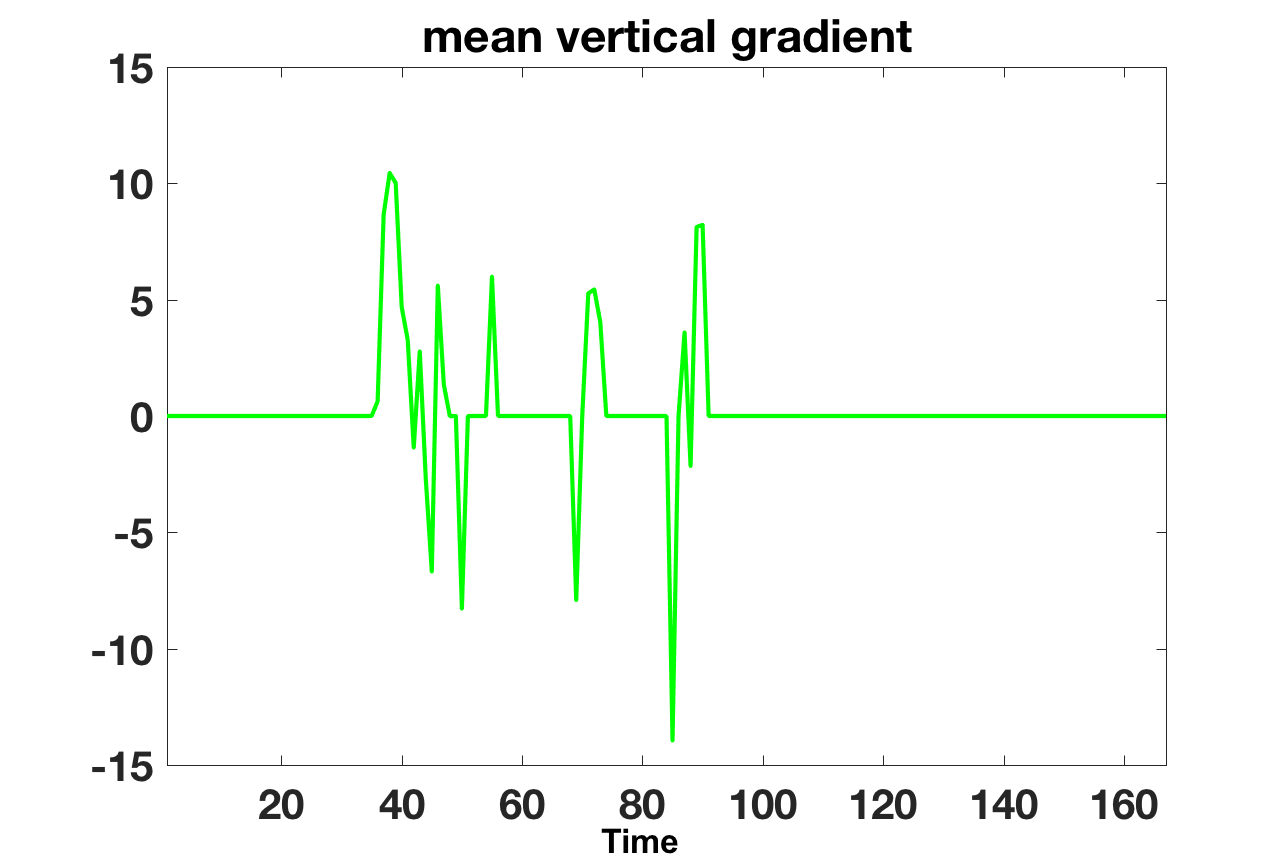
\includegraphics[scale=0.52]{images/quickoutandin.png}
\caption{Mean vertical gradient for two people walking in together}
\label{together}
\end{figure}

\begin{figure}[!htb]
\centering
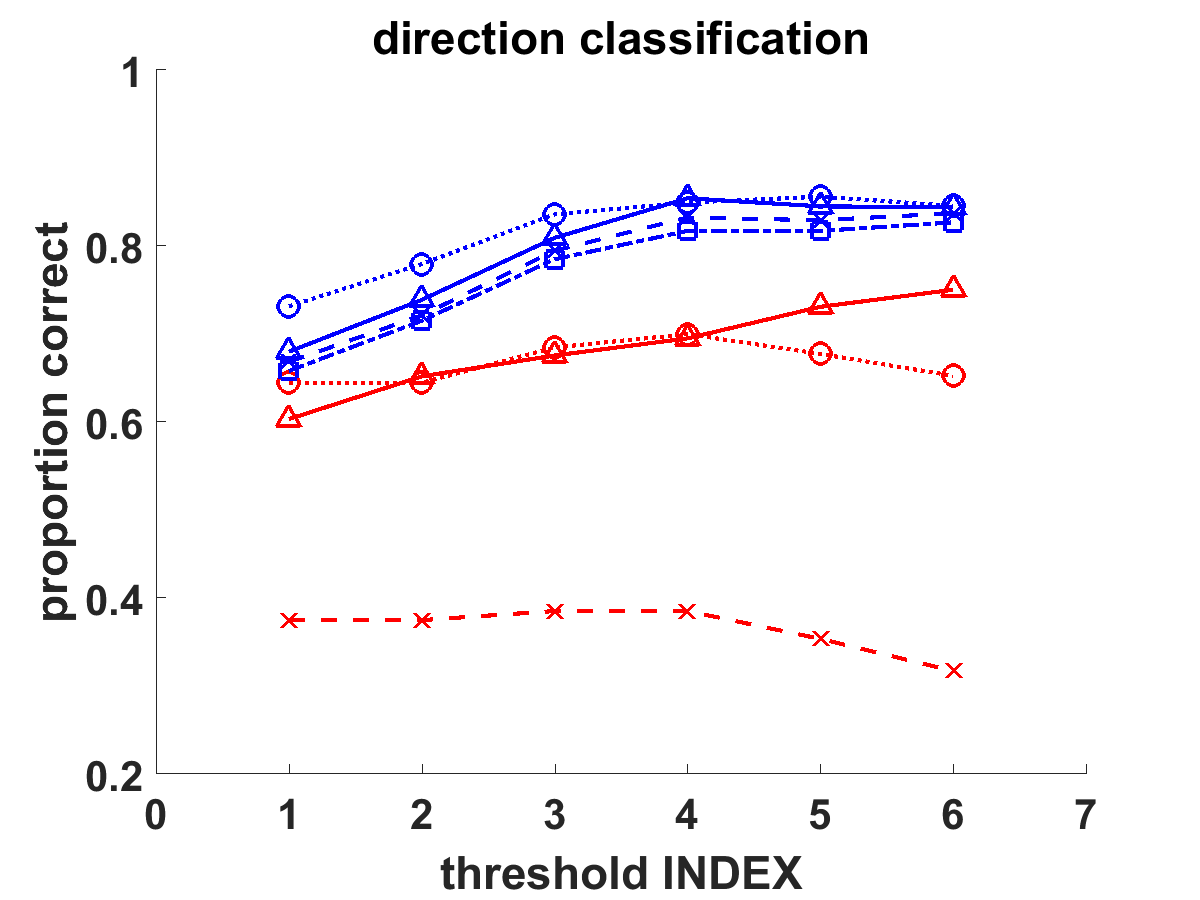
\includegraphics[scale=0.4]{images/dirClass.png}
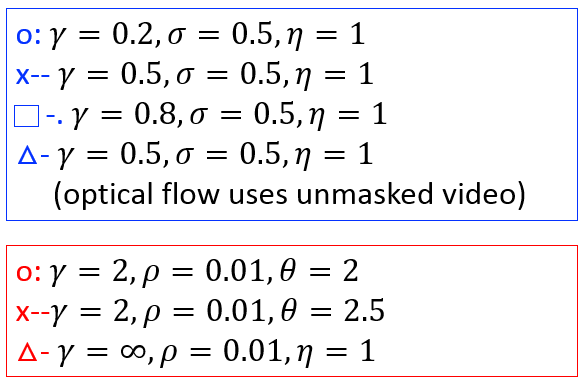
\includegraphics[scale=0.4]{images/legend.png}
\caption{Proportion of correct direction classifications with peak peformance at ~90\%.}
\label{dirclass}
\end{figure}

\begin{figure}[!htb]
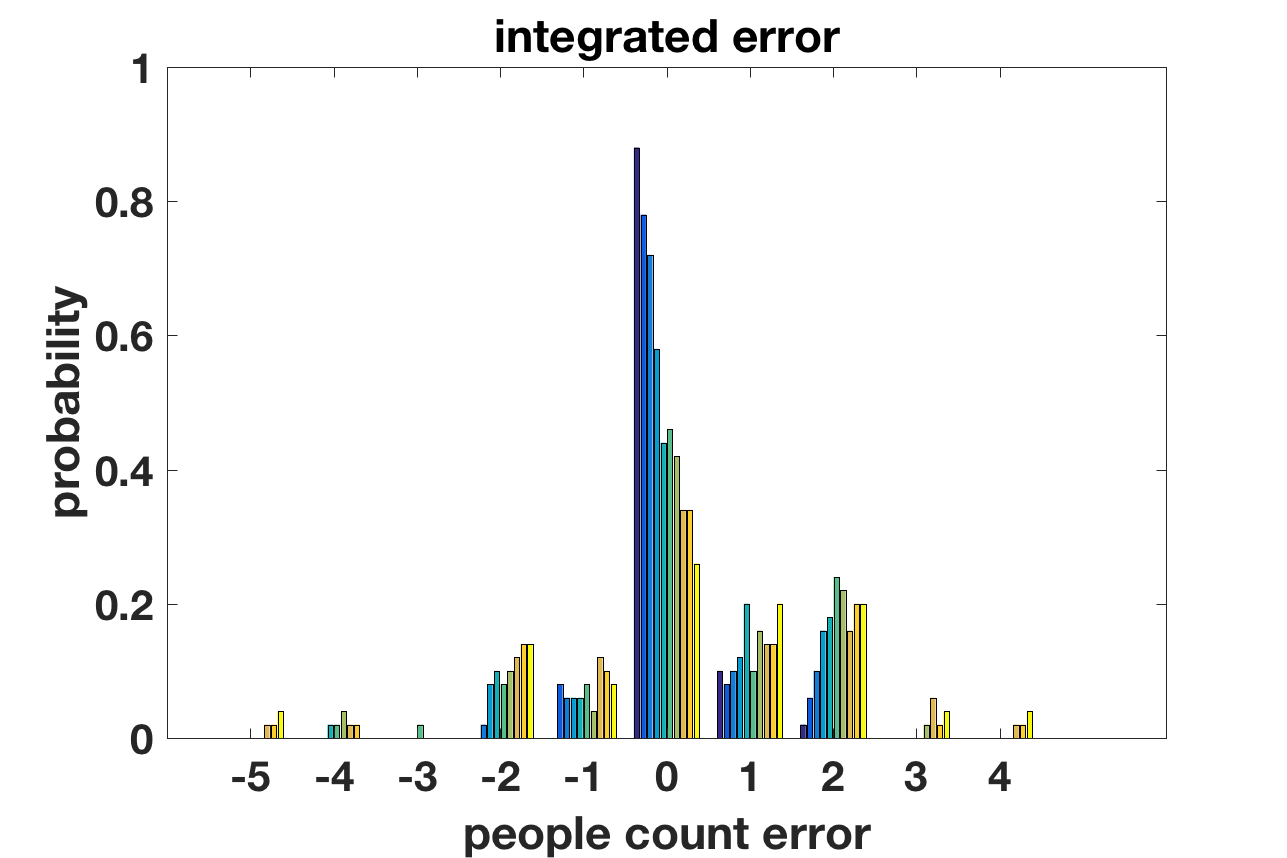
\includegraphics[scale=0.35]{images/pcerror_gamma020_hist.png}
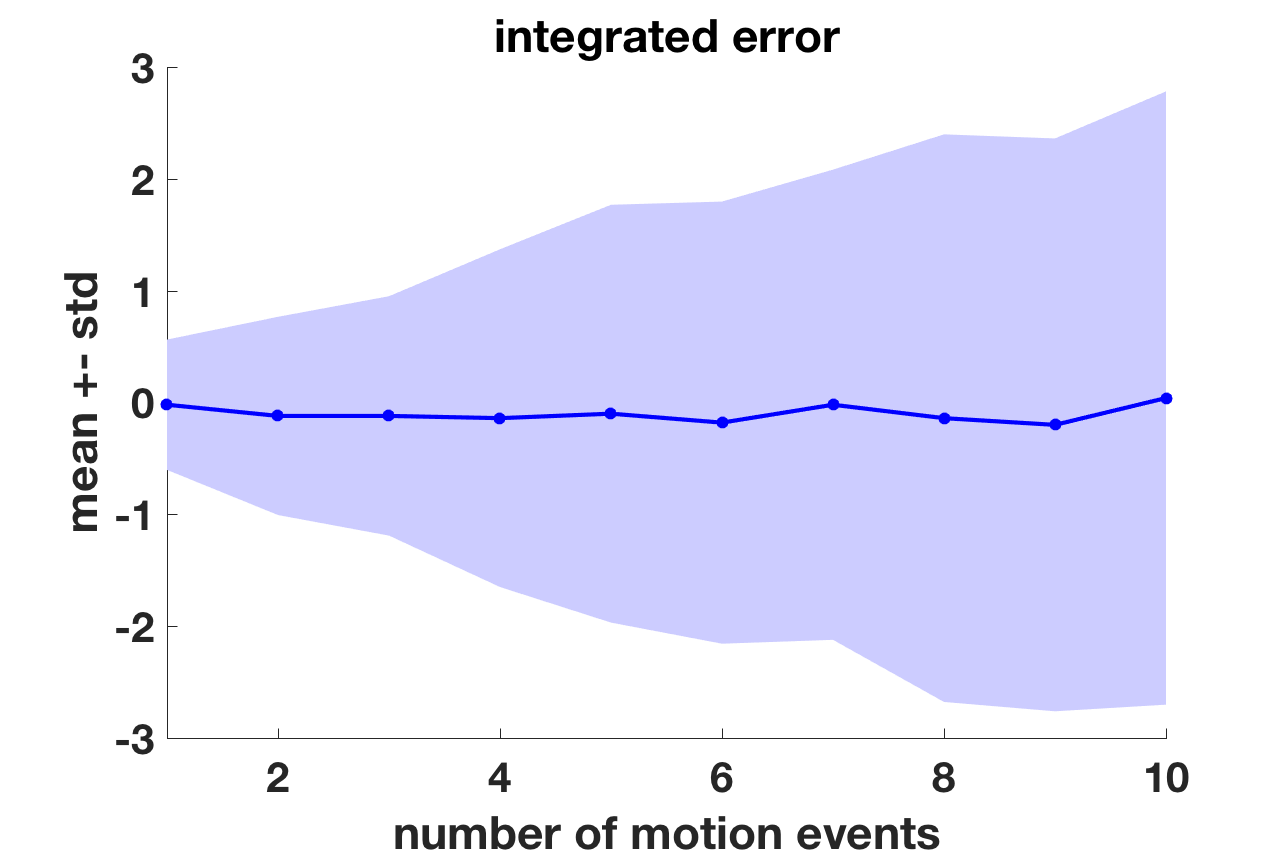
\includegraphics[scale=0.35]{images/pcerror_gamma020.png}
\caption{(LEFT) Histogram of people count errors after 1 motion event (blue) to 10 motion events (yellow). (RIGHT) The same distribution of errors shown as mean (solid line) and standard deviation (shaded region) as the number of motion events increases.}
\label{hist}
\end{figure}

\clearpage
\subsection{People Count}
Room occupancy is computed as cumulative sum of people entering and exiting the room. Since the errors here
integrate, we find that the variance of the error is quite large after only several motion events.
The standard deviation of the error after 10 events is up to 3 (Figure~\ref{hist}).


\section{Conclusions} % Should become Conclusions
% Describe what you have learned from the project and what further improvements are possible.
Although these algorithms perform well in capturing individual motion events, the resulting integrated people count is 
not a reliable estimate of room occupancy. There are several possible ways that this method could be improved. The
first is to increase the frame rate of the thermal sensors to improve capture of fast motion and gaps between 
two people passing through the door in quick succession. This could also result in a different distribution of 
background noise but this can be dealt with by preprocessing the data or by the background model. Secondly,
the detection of motion events could be improved to split single events that are suggestive of multiple people
For example, when two people pass through quickly, one event is labeled but there are two clear peaks in the
number of detected pixels. Finally, this split could also occur in the direction detection state where zero crossings
of the vertical gradient indicate a person passing through the doorway. In addition, logically the next step would be
to implement the algorithms in real-time.

% Plots (PostScript files) are included through the ``figure'' environment.
% For more complicated figures use the minipage commaned (see LaTeX manual).
% --------------------------------------------------------------------------
%%\begin{figure}[htb]
%%%
%%  \begin{minipage}[t]{0.49\linewidth}\centering
%%%    \centerline{\epsfig{figure=figures/regbsdcod.eps,width=8.0cm}}
%%    \Ovalbox{\vbox to 1.5in{\vfill\hbox{\vtop{\hsize=2.5in\hfill}\hfill}\vfill}}
%%    \medskip
%%    \centerline{(a)}
%%  \end{minipage}\hfill
%%%
%%  \begin{minipage}[t]{0.49\linewidth}\centering
%%%    \centerline{\epsfig{figure=figures/regbsdcod.eps,width=8.0cm}}
%%    \Ovalbox{\vbox to 1.5in{\vfill\hbox{\vtop{\hsize=2.5in\hfill}\hfill}\vfill}}
%%    \medskip
%%    \centerline{(b)}
%%  \end{minipage}
%%
%%  \bigskip
%%
%%  \begin{minipage}[t]{0.49\linewidth}\centering
%%%    \centerline{\epsfig{figure=figures/regbsdcod.eps,width=8.0cm}}
%%    \Ovalbox{\vbox to 1.5in{\vfill\hbox{\vtop{\hsize=2.5in\hfill}\hfill}\vfill}}
%%    \medskip
%%    \centerline{(c)}
%%  \end{minipage}\hfill
%%%
%%  \begin{minipage}[t]{0.49\linewidth}\centering
%%%    \centerline{\epsfig{figure=figures/regbsdcod.eps,width=8.0cm}}
%%    \Ovalbox{\vbox to 1.5in{\vfill\hbox{\vtop{\hsize=2.5in\hfill}\hfill}\vfill}}
%%    \medskip
%%    \centerline{(d)}
%%  \end{minipage}
%%%
%%  \caption{Block diagram: (a) one; (b) two; (c) three, and (d) four.}
%%  \label{fig:example}
%%\end{figure}

% Bibliography.
% -------------
\parskip=0pt
\parsep=0pt
\clearpage
\bibliographystyle{ieeetrsrt}

% Important: substitute your BiBTeX (*.bib) files below.
% ------------------------------------------------------
\bibliography{strings,konrad,manuals}



\end{document}
